\chapter{SpdyProxyPython}
\label{spdyproxypython}

\section{Introducci'on}

A lo largo de los cap'itulos anteriores, hemos visto, el crecimiento de Internet, en el Cap'itulo \ref{desarrolloWeb}, las deficiencias de los protocolos, en el Cap'itulo \ref{protocolos}, y la problem'atica de los tiempos de carga y sus posibles optimizaciones en el Cap'itulo \ref{problematica}. Tambi'en se ha visto SPDY como propuesta a resolver varios de los problemas actuales de la carga de los sitios, pero tambi'en, en ciertos contextos no funciona como lo esperado \ref{}. Por todo ello, se desarroll'o un Proxy (ver Cap'itulo \ref{proxy}), cuya funcionalidad principal es seleccionar de los m'etodos habilitados que ofrezca un sitio (HTTP HTTPS, SPDY) cu'al es el m'as 'optimo para recuperar el recurso. Posee otras funcionalidades tales como, ser MITM\footnote{Man in The Middle}, Cach'e (ver Cap'itulo \ref{cache}), c'alculo de RTT, recuperaci'on de los m'etodos habilitados para un sitio, cliente SPDY.

Se eligi'o Python\footnote{https://www.python.org/} como lenguaje y MongoDB\footnote{http://http://www.mongodb.org/} para el almacenamiento de los datos de los sitios.

\section{Funcionamiento}

El Proxy se inicia en una direcci'on y en un puerto, por ejemplo: \textit{localhost:8080} se debe configurar el Navegador para que utilice la direcci'on del proxy para conectarse a Internet. Por ejemplo en Google Chrome se puede iniciar con un Flag para configurar el proxy:
\begin{quote}
\textit{chrome --proxy-server="localhost:8080"}
\end{quote}
Acepta tanto conexiones HTTP, como HTTPS en el mismo puerto. Al realizar la conexi'on por SSL con el cliente en vez de actuar de ''puente'' con el destino final, utiliza un Certificado SSL para realizar la autenticaci'on.

Cuando recibe una petici'on HTTP, el m'etodo que llega al Proxy es \textit{GET}, se consulta la Cach'e para ver si el recurso se encuentra almacenado para retornarlo desde la copia del Proxy, si no se encuentra, se pide al servidor correspondiente y se devuelve el recurso al cliente. Luego, se realiza el An'alisis del Recurso (ver \ref{analisisRecurso}) en segundo plano.

Cuando recibe una petici'on HTTPS, el m'etodo que llega al Proxy es CONNECT, que es un m'etodo especial para solicitarle a un Proxy una conexi'on al servidor final. En este caso, el Proxy responde con el mensaje:
\begin{quote}
\textit{\textit{HTTP/1.1 200 Connection established}}
\end{quote}
Para indicarle que se va a realizar la conexi'on. Esta primera etapa puede verse en la Figura \ref{mitm1}.

\begin{figure}[h]
  	\centering
	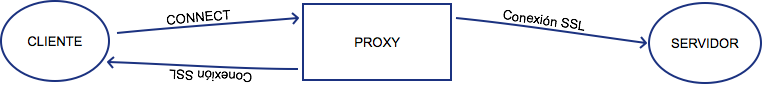
\includegraphics[width=\textwidth]{img/mitm1}
	\caption{\small Conexi'on inicial cuando el protocolo es HTTPS}
	\label{mitm1}
\end{figure}

Luego, se inicia la conexi'on SSL Cliente-Proxy y comienzan a recibirse las peticiones del Cliente, como puede verse en la Figura \ref{mitm2}, las conexiones\footnote{Tanto hacia el Cliente como hacia el Servidor.} se realizan individualmente (no como un T'unel HTTPS normal, ver Figura \ref{proxy_2}). Con cada una de las peticiones, se procede de manera similar a HTTP. Se analiza si el recurso se encuentra almacenado en la cach'e y se devuelve de la copia local, o se solicita el recurso al servidor final. En el caso de que el m'etodo seleccionado para devolver el recurso sea HTTS o SPDY, se establece una conexi'on segura entre el proxy y el servidor final.

Cabe destacar que, todo el tr'afico que fluye entre el cliente y el proxy, y entre el proxy y el servidor final, viaja encriptado. Pero, todo el tr'afico se encuentra desencriptado en el Proxy, siendo un proxy HTTPS de confianza.

\begin{figure}[h]
  	\centering
	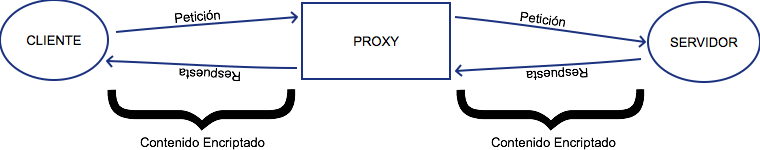
\includegraphics[width=\textwidth]{img/mitm2}
	\caption{\small Procedimiento una vez realizada la conexi'on en los 2 extremos}
	\label{mitm2}
\end{figure}

\subsection{An'alisis de los Recursos}
\label{analisisRecurso}
Cada vez que el Proxy recibe una petici'on del cliente, se analiza si el recurso se encuentra en la Cach'e, en el caso de que el recurso se encuentre almacenado, se devuelve desde la copia local del Proxy y se actualiza la Cach'e con el Hit del elemento correspondiente. Caso contrario, se peticiona el recurso servidor final.
Cada vez que el Proxy pide un recurso, se realiza un an'alisis del mismo en segundo plano:
\begin{enumerate}
\item C'alculo del RTT: se realiza el c'alculo del RTT al host donde se aloja el recurso.
\item Obtenci'on de Protocolos: Se obtienen los protocolos soportados (HTTP, HTTPS, SPDY) del host donde se aloja el recurso.
\item C'alculo de Peticiones a Generar: en el caso de que el recurso sea un HTML plano, se calcula cuantas peticiones generar'ia. Se realiza analizando el texto y extrayendo los recursos que esa p'agina va a necesitar para su renderizaci'on.
\end{enumerate}
Toda esta informaci'on, luego es consumida por el 'Arbol de Decisi'on para determinar que protocolo es el m'as 'optimo para recuperar el recurso.

\subsection{'Arbol de Decisi'on}